% arara: pdflatex
% !arara: biber
% !arara: pdflatex
% How to run: 
% 1) pdflatex "filename".tex
% 2) biber "filename"
% 3) pdflatex "filename".tex
% 4) pdflatex "filename".tex


\documentclass[x11names]{article}
\usepackage{verbatim}
\usepackage{listings}
\usepackage{graphicx}
\usepackage{a4wide}
\usepackage{color}
\usepackage{amsmath}
\usepackage{amssymb}
\usepackage[dvips]{epsfig}
\usepackage[T1]{fontenc}
% \usepackage{cite} % [2,3,4] --> [2--4]
\usepackage{shadow}
\usepackage{hyperref}
\usepackage{physics}
\usepackage{url}
\usepackage{tikz}
\usepackage{subcaption}
\usepackage[utf8]{inputenc}
\usepackage{booktabs} % Allows the use of \toprule, \midrule and \bottomrule in tables
\usepackage[font={small,it}]{caption}
\usepackage[margin=0.7in]{geometry} %Sets the margins in the document
\usepackage{siunitx}    %Allows use of SI units macros

%Defines calculator way to write powers of ten
\sisetup{output-exponent-marker=\textsc{e}}
%Physics package had ugly vectors
\renewcommand{\va}{\vec}
% Change numbering and some commands
\renewcommand\thesection{Exercise \arabic{section}}
\renewcommand\thesubsection{\Roman{section}.\alph{subsection}}

%% references
\usepackage[style=authoryear,
            bibstyle=authoryear,
            backend=biber,
            % refsection=chapter,
            maxbibnames=99,
            maxnames=2,
            firstinits=true,
            uniquename=init,
            natbib=true,
            dashed=false]{biblatex}

\addbibresource{bibliography.bib}
% \addbibresource{top.bib}

% \bibliography{bibliography}
% \bibliography{top}


\usepackage[capitalize]{cleveref}

\setcounter{tocdepth}{2}

\lstset{language=c++}
\lstset{alsolanguage=[90]Fortran}
\lstset{basicstyle=\small}
\lstset{backgroundcolor=\color{white}}
\lstset{frame=single}
\lstset{stringstyle=\ttfamily}
\lstset{keywordstyle=\color{red}\bfseries}
\lstset{commentstyle=\itshape\color{blue}}
\lstset{showspaces=false}
\lstset{showstringspaces=false}
\lstset{showtabs=false}
\lstset{breaklines}


\definecolor{keywords}{RGB}{255,0,90}
      \definecolor{comments}{RGB}{0,0,113}
      \definecolor{red}{RGB}{160,0,0}
      \definecolor{green}{RGB}{0,150,0}
       
      \lstset{language=Python, 
              basicstyle=\ttfamily\small, 
              keywordstyle=\color{keywords},
              commentstyle=\color{comments},
              stringstyle=\color{red},
              showstringspaces=false,
              identifierstyle=\color{green}
              }

\begin{document}
  \section{}
    \begin{itemize}
      \item Should be fixed now
    \end{itemize}

  \section{}
    \begin{itemize}
      \item Fixed alot of the sloppy errors I had here
    \end{itemize}

  \section{}
    \begin{itemize}
      \item Yeah, I think RK4 should work nicely. If they get the algorithm provided it shouldn't be too hard. I'm working on rewriting the code a little to be more readable
    \end{itemize}

  \section{}
    \begin{itemize}
      \item To be done
    \end{itemize}

  \section{}
    \begin{itemize}
      \item Fixed typo
      \item I also recognized that the latitude-longitude grid presentation of the data wasn't the best so visualization. So I also implemented a orthographic map projection I just hadn't put into the reports yet, see \cref{fig:potential} and the appendix for the code. It was created much nicer countourplots, and uses basemaps (som python module) to create the northen hemisphere map. I was thinking that it code snippet to create a basemap it should be quite easy for them to use that to draw their contourplot onto.
    \end{itemize}

    \begin{figure}
      \centering
      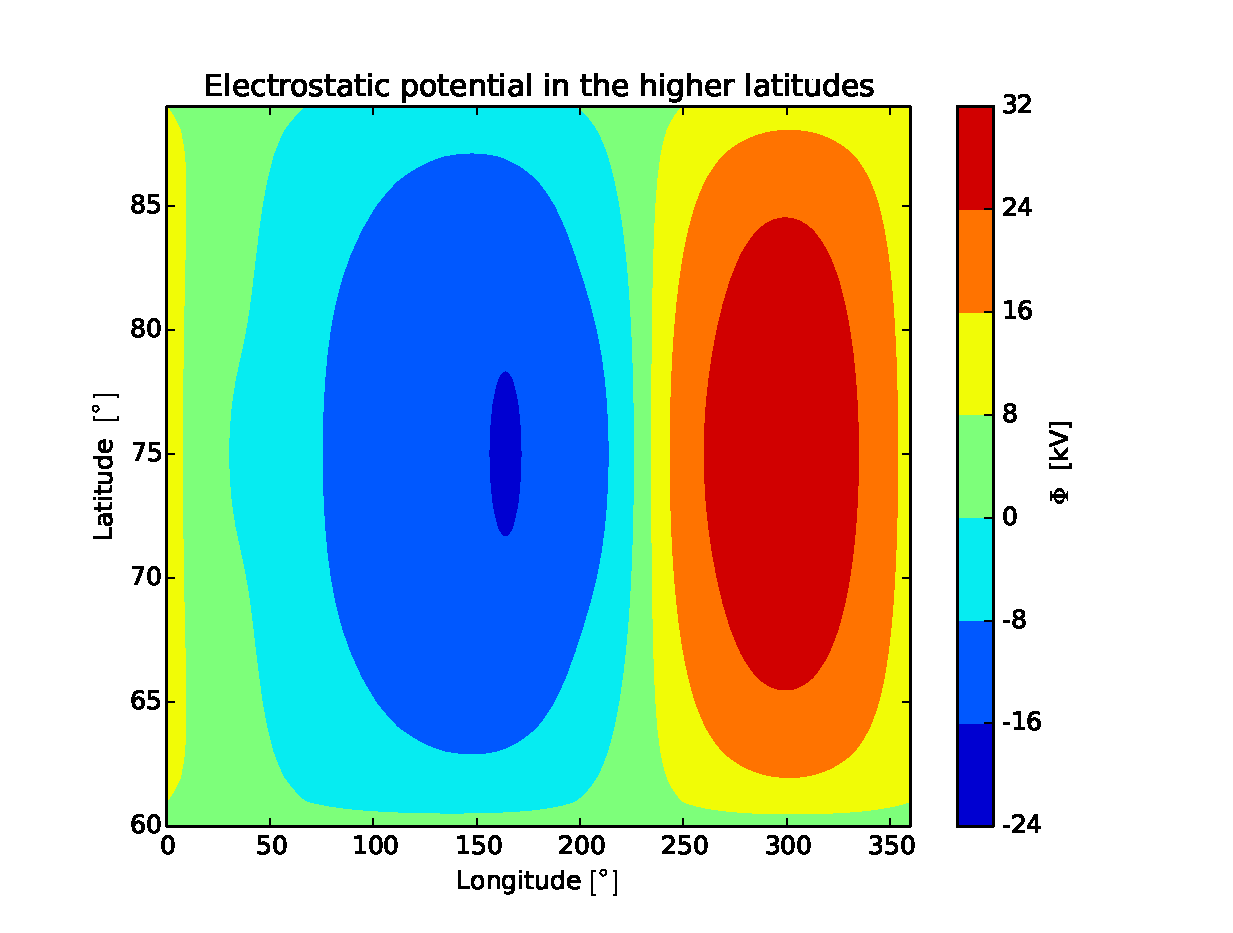
\includegraphics[width = 0.30\textwidth]{potential}
      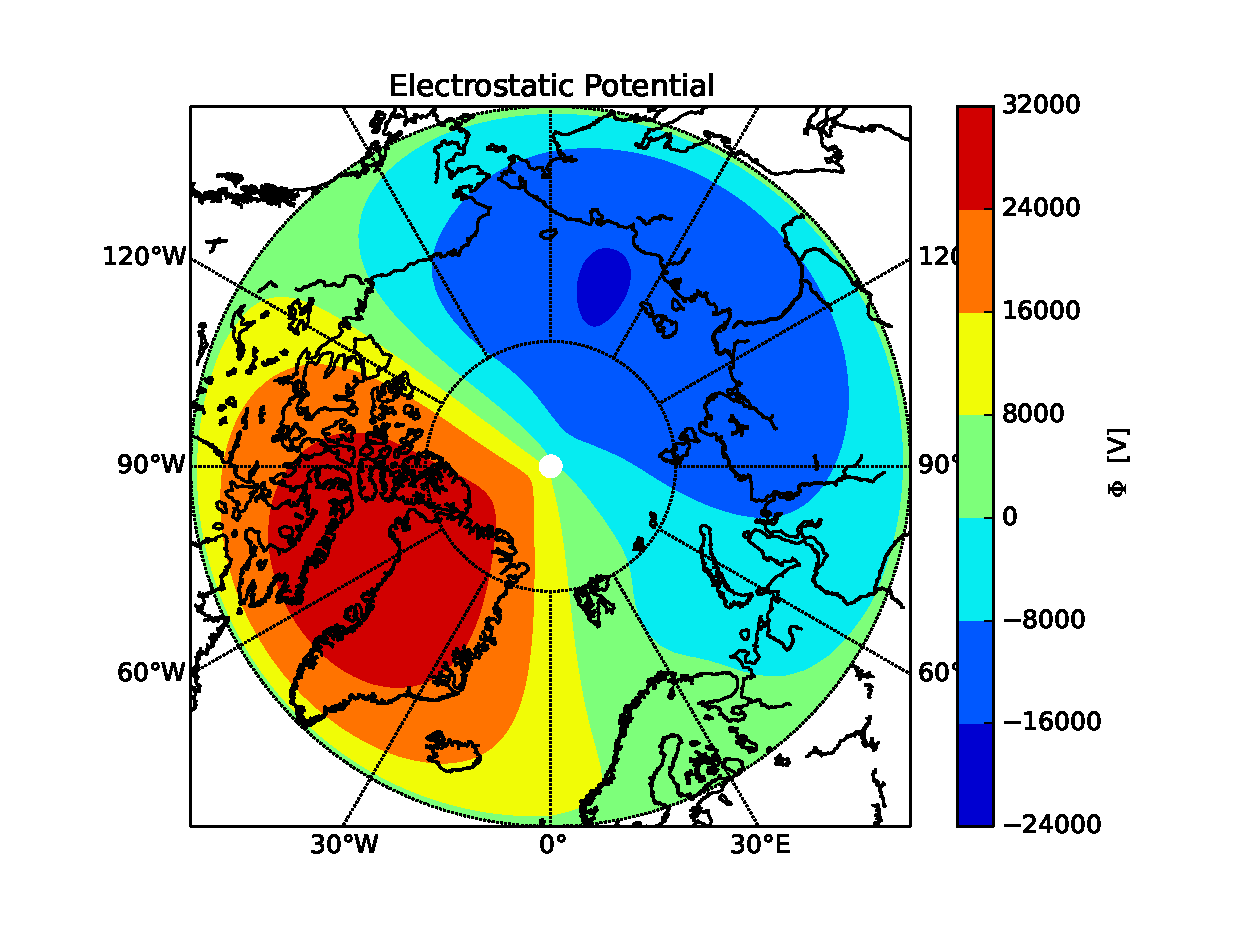
\includegraphics[width = 0.30\textwidth]{map_potential}
      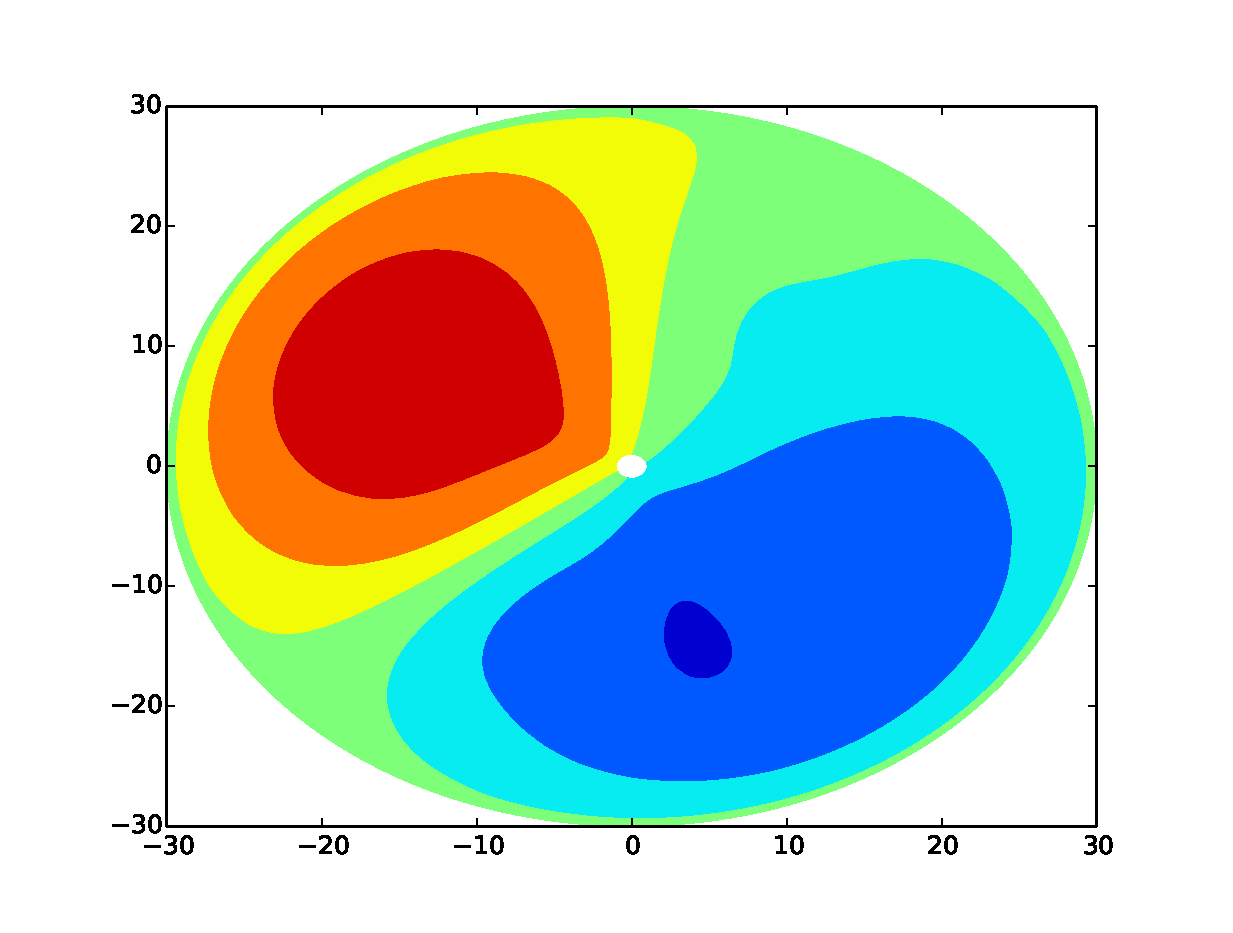
\includegraphics[width = 0.30\textwidth]{other_proj}
      \caption{The electrostatic potential, left figure is with latitude-longitude grid, center figure is an orthographic projection, right figure is a simplified stereographic projection}
      \label{fig:potential}
    \end{figure}

  \section{}
    \begin{itemize}
      \item Also had a map projection of the vector field see \cref{fig:drift}.
    \end{itemize}

    \begin{figure}
      \centering
      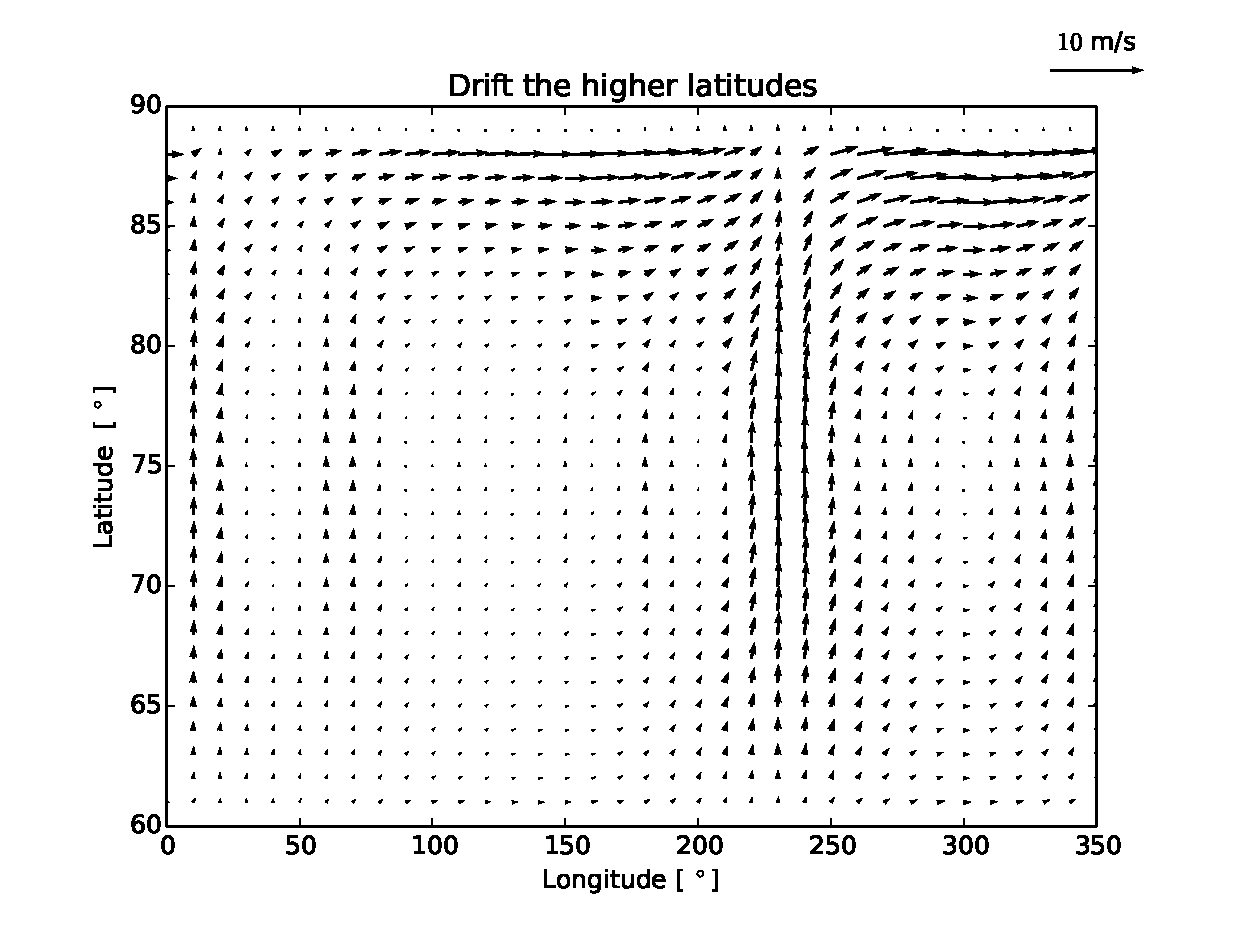
\includegraphics[width = 0.45\textwidth]{vArrows}
      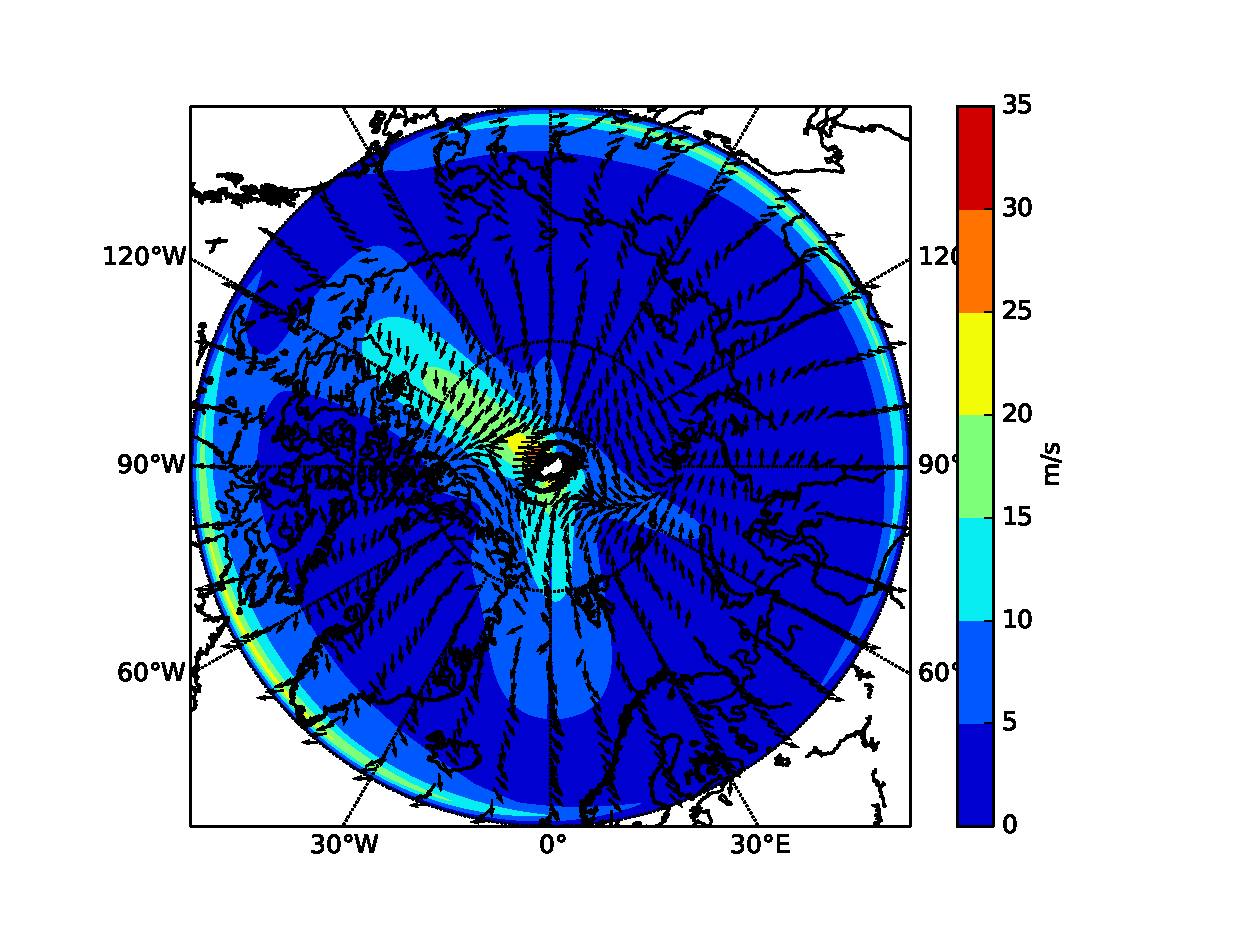
\includegraphics[width = 0.45\textwidth]{map_drift}
      \caption{E\(\cross\)B drift}
      \label{fig:drift}
    \end{figure}

  \appendix
  \section{}
  Code located in github folder 'Exercise\_7/source/draw\_map.py'
  \lstinputlisting{../Exercise_7/source/draw_map.py}
  
\end{document}